\usetikzlibrary{arrows}
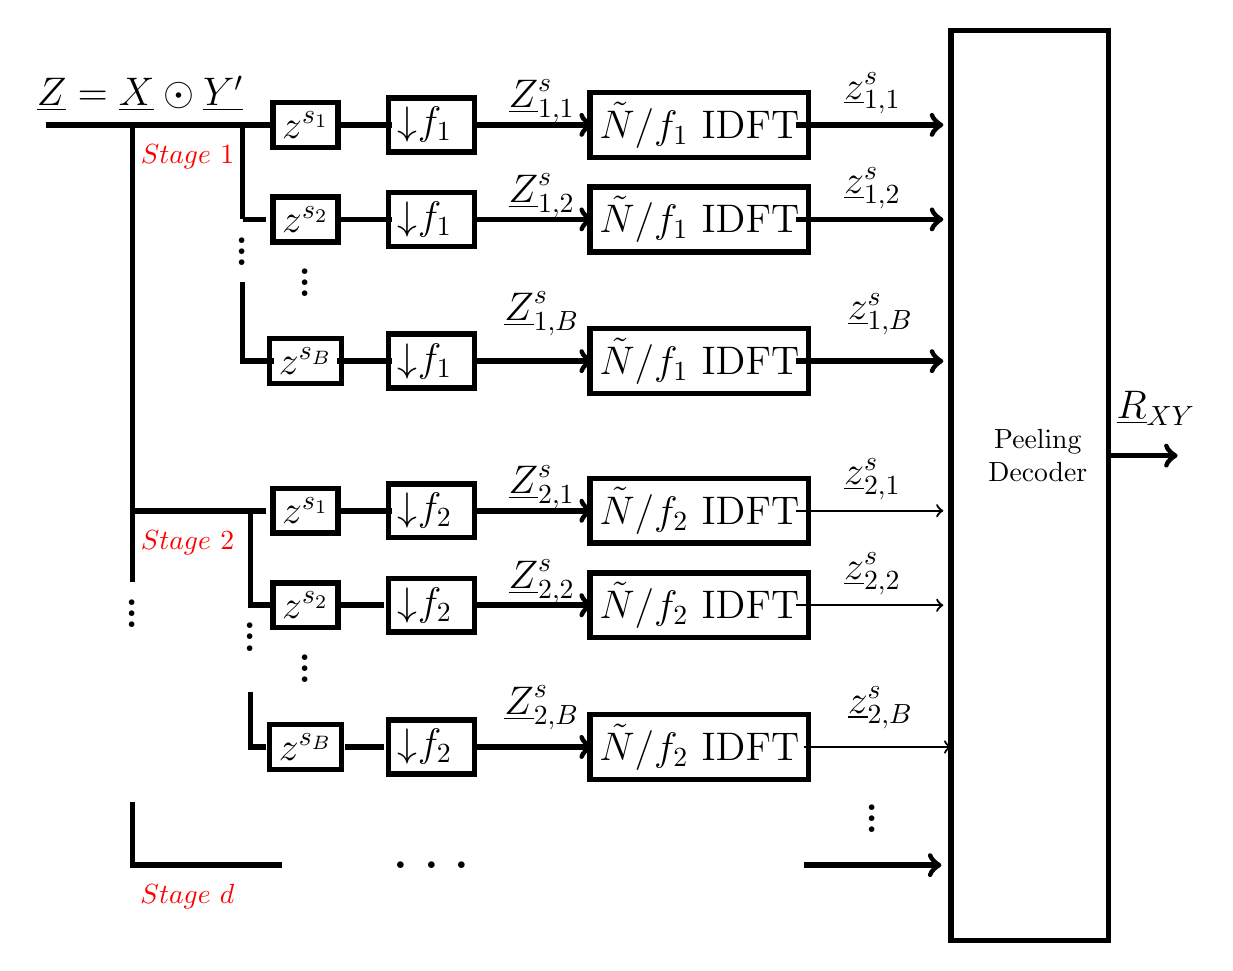
\begin{tikzpicture}

 % Downsampling blocks
\node[draw,align=center,thick,line  width =2pt] at (1.8,4.5) {\Large{$\mathbf{\downarrow} f_2$} };
\node[draw,align=center,thick,line  width =2pt] at (1.8,5.7) {\Large{$\mathbf{\downarrow} f_2$ }};
\node[draw,align=center,thick,line  width =2pt] (v6) at (1.8,2.7) {\Large{$\mathbf{\downarrow} f_2$ }};

\node[draw,align=center,thick,line  width =2pt] at (1.8,9.4) {\Large{$\mathbf{\downarrow} f_1$} };
\node[draw,align=center,thick,line  width =2pt] at (1.8,10.6) {\Large{$\mathbf{\downarrow} f_1$ }};
\node[draw,align=center,thick,line  width =2pt] at (1.8,7.6) {\Large{$\mathbf{\downarrow} f_1$ }};

%  Input lines to the down-sampling block

 
  
 


%  Delay blocks

\node[draw,align=center,thick,line  width =2pt] at (0.2,10.6) {\bf \Large{$z^{s_1}$}};
\node[draw,align=center,thick,line  width =2pt] at (0.2,9.4) {\bf \Large{$z^{s_2}$}};
\node[draw,align=center,thick,line  width =2pt] at (0.2,7.6) {\bf \Large{$z^{s_B}$}};

\node[draw,align=center,thick,line  width =2pt] at (0.2,5.7) {\bf \Large{$z^{s_1}$}};
\node[draw,align=center,thick,line  width =2pt] at (0.2,4.5) {\bf \Large{$z^{s_2}$}};
\node[draw,align=center,thick,line  width =2pt] at (0.2,2.7) {\bf \Large{$z^{s_B}$}};




% paths connecting the delay blocks
 
 
 
 \draw[thick,line  width =2pt] (1.3,9.4) -- (0.6,9.4);
 

\node[line  width =2pt] at (-0.6,9.1) {\Huge${\vdots}$};
\node[line  width =2pt] at (0.2,8.7) {\Huge${\vdots}$};
\node[line  width =2pt] at (-0.5,4.2) {\Huge${\vdots}$};
\node[line  width =2pt] at (0.2,3.8) {\Huge${\vdots}$};

 \draw[thick,line  width =2pt] (1.3,10.6) -- (0.6,10.6);
 \draw[thick,line  width =2pt] (-0.6,9.4) -- (-0.6,10.6);
 
% paths connecting the two stages   
 \draw[thick,line  width =2pt] (-0.2,10.6) -- (-2,10.6);
 \draw[thick,line  width =2pt] (-0.6,9.4) -- (-0.3,9.4);
 \draw[thick,line  width =2pt] (-0.3,5.7) -- (-2,5.7);
 \draw[thick,line  width =2pt] (-2,5.7) -- (-2,10.6);
  \draw[thick,line  width =2pt] (-3.1,10.6) -- (-2,10.6);
  \draw[thick,line  width =2pt] (-2,5.7) -- (-2,4.8);
  
  
  % DFT blocks
\node[draw,align=center,thick,line  width =2pt] at (5.2,4.5) {\Large{$\tilde{N}/f_2$ IDFT}};
\node[draw,align=center,thick,line  width =2pt] at (5.2,5.7) {\Large{$\tilde{N}/f_2$ IDFT}};
\node[draw,align=center,thick,line  width =2pt] at (5.2,2.7) {\Large{$\tilde{N}/f_2$ IDFT}};

\node[draw,align=center,thick,line  width =2pt] at (5.2,9.4) {\Large{$\tilde{N}/f_1$ IDFT}};
\node[draw,align=center,thick,line  width =2pt] at (5.2,10.6) {\Large{$\tilde{N}/f_1$ IDFT}};
\node[draw,align=center,thick,line  width =2pt] at (5.2,7.6) {\Large{$\tilde{N}/f_1$ IDFT}};
% Connectors
 \draw[->,thick,line  width =2pt] (2.35,10.6) -- (3.85,10.6);
 \draw[->,thick,line  width =2pt] (2.35,9.4) -- (3.85,9.4);
 \draw[->,thick,line  width =2pt] (2.35,7.6) -- (3.85,7.6);
 
 \draw[->,thick,line  width =2pt] (2.35,5.7) -- (3.85,5.7);
 \draw[->,thick,line  width =2pt] (2.35,4.5) -- (3.85,4.5);
 \draw[->,thick,line  width =2pt] (2.35,2.7) -- (3.85,2.7);

 \draw[->,thick,line  width =2pt] (6.43,10.6) -- (8.3,10.6);
 \draw[->,thick,line  width =2pt] (6.43,9.4) -- (8.3,9.4);
 \draw[->,thick,line  width =2pt] (6.43,7.6) -- (8.3,7.6);
 
 \draw[->,thick] (6.43,5.7) -- (8.3,5.7);
 \draw[->,thick] (6.43,4.5) -- (8.3,4.5);
 \draw[->,thick] (6.53,2.7) -- (8.4,2.7);
 
  % Labels
  \node[draw=none,align=center] at (-1.9,11) {\Large{$\underline{Z}= \underline{X} \odot \underline{Y'}$}};
  
  \node[draw=none,align=center] at (3.2,10.9) {\Large{$\underline{Z}^{s}_{1,1}$}};
  \node[draw=none,align=center] at (3.2,9.7) {\Large{$\underline{Z}^{s}_{1,2}$}};
\node[draw=none,align=center] at (3.2,8.2) {\Large{$\underline{Z}^{s}_{1,B}$}};

\node[draw=none,align=center] at (3.2,6) {\Large{$\underline{Z}^{s}_{2,1}$}};
  \node[draw=none,align=center] at (3.2,4.8) {\Large{$\underline{Z}^{s}_{2,2}$}};
  \node[draw=none,align=center] at (3.2,3.2) {\Large{$\underline{Z}^{s}_{2,B}$}};

  \node[draw=none,align=center] at (7.4,11) {\Large{$\underline{z}^{s}_{1,1}$}};
  \node[draw=none,align=center] at (7.4,9.8) {\Large{$\underline{z}^{s}_{1,2}$}};
  \node[draw=none,align=center] at (7.5,8.2) {\Large{$\underline{z}^{s}_{1,B}$}};
  
  \node[draw=none,align=center] at (7.4,6.1) {\Large{$\underline{z}^{s}_{2,1}$}};
  \node[draw=none,align=center] at (7.4,4.9) {\Large{$\underline{z}^{s}_{2,2}$}};
  \node[draw=none,align=center] at (7.5,3.2) {\Large{$\underline{z}^{s}_{2,B}$}};
  
  \node [draw=none] at (-2,4.5) {\Huge${\vdots}$} ;
  
   \node[draw=none,align=center] at (-1.3,10.2) {\color{red}$Stage ~1$};
  \node[draw=none,align=center] at (-1.3,5.3) {\color{red}$Stage ~2$};
   \node[draw=none,align=center] at (-1.3,0.8) {\color{red}$Stage ~d$};
\draw [thick,line  width =2pt](-2,2) -- (-2,1.2) -- (-0.1,1.2) ;
 \node[draw=none,align=center] at (1.8,1.2) {\Huge${\ldots}$};
 
\draw [thick,line  width =2pt] (8.4,0.2424) rectangle (10.4,11.8);
\node (v1) at (6.4,1.2) {};
\node (v2) at (8.4,1.2) {};



\node (v11) at (1.3,7.6) {};


\draw  [->,thick,line  width =2pt](v1) edge (v2);
\node at (7.4,1.9) {\Huge${\vdots}$};
\node [text width=3cm, align =center ] at (9.5,6.4) {Peeling \\ Decoder};
\node (v3) at (10.3,6.4) {};
\node (v4) at (11.4,6.4) {};
\draw [thick, ->,line  width =2pt] (v3) edge (v4);
\node at (11,7) {\Large{$\underline{R}_{XY}$}};







\draw[thick,line  width =2pt] (-0.6,8.6) -- (-0.6,7.6) -- (-0.2,7.6);
\draw[thick,line  width =2pt] (0.6,7.6) -- (1.3,7.6);
\draw[thick,line  width =2pt] (-0.5,5.7) -- (-0.5,4.5) -- (-0.2,4.5);
\draw[thick,line  width =2pt] (-0.5,3.4) -- (-0.5,2.7) -- (-0.3,2.7);
\draw [thick,line  width =2pt](0.6,5.7) -- (1.3,5.7);
\draw[thick,line  width =2pt] (0.6,4.5) -- (1.2,4.5);
\draw[thick,line  width =2pt] (0.7,2.7) -- (1.2,2.7);
\end{tikzpicture}